%%%%%%%%%%%%%%%%%%%%%%%%%%%%%%%%%%%%%%%%%
%% Appendix section
% Set-up the section.
%\newpage
\onehalfspacing
\appendix
\setcounter{table}{0}
\renewcommand{\thetable}{A\arabic{table}}
\setcounter{figure}{0}
\renewcommand{\thefigure}{A\arabic{figure}}

% Start appendix
\section{Appendix}
\label{appendix}
% This project used computational tools which are fully open-source.
%As such, all code and data involved in this project are available at this project's Github repository, available at \url{https://github.com/shoganhennessy/state-faculty-composition}.
%They may be used for replication, or as the basis for further work, as needed.
Any comments or suggestions may be sent to me at \href{mailto:seh325@cornell.edu}{\nolinkurl{seh325@cornell.edu}}, or raised as an issue on the Github project.

\subsection{Identification in Causal Mediation}
\label{appendix:identification}
\citet[Theorem~1]{imai2010identification} states that the ADE and AIE are identified under sequential ignorability, at each level of $Z_i = 0,1$.
For $z' = 0,1$: \\
\makebox[\textwidth]{\parbox{1.25\textwidth}{
\begin{align*}
    \E{ Y_i(1, D_i(z')) - Y_i(0, D_i(z'))}
    &= \int \int 
    \Big( \Egiven{ Y_i }{Z_i = 1, D_i, \vec X_i}
        - \Egiven{ Y_i }{Z_i = 0, D_i, \vec X_i} \Big)
            dF_{D_i \, | \, Z_i = z', \vec X_i} dF_{\vec X_i}, \\
    \E{ Y_i(z', D_i(1)) - Y_i(z', D_i(0))}
    &= \int \int \Egiven{ Y_i }{Z_i = z', D_i, \vec X_i}
    \Big( dF_{D_i \, | \, Z_i = 1, \vec X_i}
        - dF_{D_i \, | \, Z_i = 0, \vec X_i} \Big) dF_{\vec X_i}.
\end{align*}
}}
I focus on the averages, which are identified by consequence of the above.
\begin{align*}
    \E{ Y_i(1, D_i(Z_i)) - Y_i(0, D_i(Z_i))}
    &= \E[Z_i]{\Egiven{ Y_i(1, D_i(z')) - Y_i(0, D_i(z'))}{Z_i = z'}} \\
    \E{ Y_i(Z_i, D_i(1)) - Y_i(Z_i, D_i(0))}
    & = \E[Z_i]{\Egiven{ Y_i(z', D_i(1)) - Y_i(z', D_i(0))}{Z_i = z'}}
\end{align*}
My estimand for the ADE is a simple rearrangement of the above.
The estimand for the AIE relies on a different sequence, relying on (1) sequential ignorability, (2) conditional monotonicity.
These give (1) identification equivalence of AIE local to cpmpliers conditional on $\vec X_i$ and AIE conditional on $\vec X_i$, LAIE $=$ AIE, (2) identification of the complier score.
%, $\Probgiven{D_i(1) = 1, D_i(0) = 0}{\vec X_i}$ $= \Egiven{Y_i}{Z_i, D_i = 1, \vec X_i}
%- \Egiven{Y_i}{Z_i, D_i = 0, \vec X_i}$.
\begin{align*}
    & \Egiven{ Y_i(Z_i, D_i(1)) - Y_i(Z_i, D_i(0))}{\vec X_i} \\
    & = \Probgiven{D_i(1) = 1, D_i(0) = 0}{\vec X_i}
        \Egiven{ Y_i(Z_i, 1) - Y_i(Z_i, 0)}{D_i(1) = 1, D_i(0) = 0, \vec X_i} \\
    & = \Probgiven{D_i(1) = 1, D_i(0) = 0}{\vec X_i}
        \Egiven{ Y_i(Z_i, 1) - Y_i(Z_i, 0)}{\vec X_i} \\
    & = \Probgiven{D_i(1) = 1, D_i(0) = 0}{\vec X_i}
        \; \Big( \Egiven{Y_i}{Z_i, D_i = 1, \vec X_i}
            - \Egiven{Y_i}{Z_i, D_i = 0, \vec X_i} \Big) \\
    & = \Big( \Egiven{D_i}{Z_i = 1, \vec X_i} - \Egiven{D_i}{Z_i = 0, \vec X_i}
        \Big) \;
        \Big( \Egiven{Y_i}{Z_i, D_i = 1, \vec X_i}
            - \Egiven{Y_i}{Z_i, D_i = 0, \vec X_i} \Big)
\end{align*}
Monotonicity is not technically required for the above.
Breaking monotonicity would not change the identification in any of the above; it would be the same except replacing the complier score with a complier/defier score, $\Probgiven{D_i(1) \neq D_i(0)}{\vec X_i} = \Egiven{D_i}{Z_i = 1, \vec X_i} - \Egiven{D_i}{Z_i = 0, \vec X_i}$.

%\subsection{Continuous Average Causal Responses}
%\label{appendix:continuous}
%Section here relating the approach to the average causal response function (see e.g., Angrist Imbens JASA 1996, Andrew Bacon for DiD 2023).

% \subsection{Previous Literature}
% \label{appendix:mediation-review}
% 
% Create a table in this section that surveys previous research which employs mediation methods while having a clear causal design for $Z_i$, but not $D_i$.
%
%\begin{tabular}{l l l l l}
%    Paper & Field & Research Design for $Z_i$ & Research Design for $D_i$ & Selection bias? \\ \hline
%    Paper name 1.    
%\end{tabular}

\subsection{Bias in Mediation Estimates}
\label{appendix:mediation-bias}
Suppose that $Z_i$ is ignorable conditional on $\vec X_i$, but $D_i$ is not.

\subsubsection{Bias in Direct Effect Estimates}
To show that the conventional approach to mediation gives an estimate for the ADE with selection and group difference-bias, start with the components of the conventional estimands.
This proof starts with the relevant expectations, conditional on a specific value of $\vec X_i$.
For each $d' =0, 1$.
\begin{align*}
    \Egiven{Y_i}{Z_i = 1, D_i = d', \vec X_i}
    =& \Egiven{Y_i(1, D_i(Z_i))}{D_i(1) = d', \vec X_i}, \\
    \Egiven{Y_i}{Z_i = 0, D_i = d', \vec X_i}
    =& \Egiven{Y_i(0, D_i(Z_i))}{D_i(0) = d', \vec X_i}
\end{align*}
And so,
\begin{align*}
    &  \Egiven{Y_i}{Z_i = 1, D_i = d', \vec X_i}
    - \Egiven{Y_i}{Z_i = 0, D_i = d', \vec X_i} \\
    =& \Egiven{Y_i(1, D_i(Z_i))}{D_i(1) = d', \vec X_i}
    - \Egiven{Y_i(0, D_i(Z_i))}{D_i(0) = d', \vec X_i} \\
    =& \Egiven{Y_i(1, D_i(Z_i)) - Y_i(0, D_i(Z_i))}{D_i(1) = d', \vec X_i} \\
    &+ \Egiven{Y_i(0, D_i(Z_i))}{D_i(1) = d', \vec X_i}
        - \Egiven{Y_i(0, D_i(Z_i))}{D_i(0) = d', \vec X_i}.
\end{align*}
The final term is a sum of the ADE, conditional on $D_i(1) = d'$, and a selection bias term --- difference in baseline outcomes between the (partially overlapping) groups for whom $D_i(1) = d'$ and $D_i(0) = d'$.

To reach the final term, note the following.
\begin{align*}
    &\Egiven{Y_i(1, D_i(Z_i)) - Y_i(0, D_i(Z_i))}{\vec X_i} \\    
    =& \Egiven{Y_i(1, D_i(Z_i)) - Y_i(0, D_i(Z_i))}{D_i(1) = d', \vec X_i} \\
    &+ \Big(1 - \Probgiven{D_i(1) = d'}{\vec X_i}\Big)
    \left( \begin{aligned}
        &\Egiven{Y_i(1, D_i(Z_i)) - Y_i(0, D_i(Z_i))}{D_i(1) = d', \vec X_i} \\ 
        & - \Egiven{Y_i(1, D_i(Z_i)) - Y_i(0, D_i(Z_i))}{D_i(1) = 1 - d', \vec X_i}
    \end{aligned} \right) 
\end{align*}
The second term is the difference between the ADE and LADE local to relevant complier groups.

Collect everything together, as follows.
\begin{align*}
    &  \Egiven{Y_i}{Z_i = 1, D_i = d', \vec X_i}
    - \Egiven{Y_i}{Z_i = 0, D_i = d', \vec X_i} \\
    =& \underbrace{
        \Egiven{Y_i(1, D_i(Z_i)) - Y_i(0, D_i(Z_i))}{\vec X_i}}_{
            \text{ADE, conditional on }\vec X_i} \\
    &+ \underbrace{
        \Egiven{Y_i(0, D_i(Z_i))}{D_i(1) = d', \vec X_i}
            - \Egiven{Y_i(0, D_i(Z_i))}{D_i(0) = d', \vec X_i}}_{
                \text{Selection bias}} \\
    &+ \underbrace{\Big(1 - \Probgiven{D_i(1) = d'}{\vec X_i}\Big)
    \left( \begin{aligned}
        &\Egiven{Y_i(1, D_i(Z_i)) - Y_i(0, D_i(Z_i))}{D_i(1) = 1 - d', \vec X_i} \\ 
        & - \Egiven{Y_i(1, D_i(Z_i)) - Y_i(0, D_i(Z_i))}{D_i(1) = d', \vec X_i}
    \end{aligned} \right)}_{
        \text{group difference-bias}}
\end{align*}
The proof is achieved by applying the expectation across $D_i = d'$, and $\vec X_i$.

\subsubsection{Bias in Indirect Effect Estimates}
To show that the conventional approach to mediation gives an estimate for the AIE with selection and group difference-bias, start with the definition of the ADE --- the direct effect among compliers times the size of the complier group.

This proof starts with the relevant expectations, conditional on a specific value of $\vec X_i$.
\begin{align*}
    &\Egiven{ Y_i(Z_i, D_i(1)) - Y_i(Z_i, D_i(0))}{\vec X_i} \\
    =& \Probgiven{D_i(1) = 1, D_i(0) = 0}{\vec X_i}
        \Egiven{ Y_i(Z_i, 1) - Y_i(Z_i, 0)}{D_i(1) = 1, D_i(0) = 0, \vec X_i}
\end{align*}
When $D_i$ is not ignorable, the bias comes from estimating the second term,\\ $\Egiven{ Y_i(Z_i, 1) - Y_i(Z_i, 0)}{D_i(1) = 1, D_i(0) = 0, \vec X_i}$.

For each $z' =0, 1$.
\begin{align*}
    \Egiven{Y_i}{Z_i = z', D_i = 1, \vec X_i}
    =& \Egiven{Y_i(z', 1)}{D_i = 1, \vec X_i}, \\
    \Egiven{Y_i}{Z_i = z', D_i = 0, \vec X_i}
    =& \Egiven{Y_i(z', 0)}{D_i = 0, \vec X_i}
\end{align*}
So compose the CM estimand, as follows.
\begin{align*}
    & \Egiven{Y_i}{Z_i = z', D_i = 1, \vec X_i}
    - \Egiven{Y_i}{Z_i = z', D_i = 0, \vec X_i} \\
    =& \Egiven{Y_i(z', 1)}{D_i = 1, \vec X_i}
        - \Egiven{Y_i(z', 0)}{D_i = 0, \vec X_i} \\
    =& \Egiven{Y_i(z', 1) - Y_i(z', 0)}{D_i = 1, \vec X_i}
    + \Egiven{Y_i(z', 0)}{D_i = 1, \vec X_i} - \Egiven{Y_i(z', 0)}{D_i = 0, \vec X_i}
\end{align*}
The final term is a sum of the AIE, among the treated group $D_i = 1$, and a selection bias term --- difference in baseline terms between the groups $D_i = 1$ and $D_i = 0$.

The AIE is the direct effect among compliers times the size of the complier group, so we need to compensate for the difference between the treated group $D_i = 1$ and complier group $D_i(1)= 1, D_i(0) = 0$.

Start with the difference between treated group's average and overall average.
\begin{align*}
    & \Egiven{Y_i(z', 1) - Y_i(z', 0)}{D_i = 1, \vec X_i} \\
    =& \Egiven{Y_i(z', 1) - Y_i(z', 0)}{\vec X_i} \\
    &+ \Big(1 - \Probgiven{D_i = 1}{\vec X_i} \Big)
    \left( \begin{aligned}
        &\Egiven{Y_i(z', 1) - Y_i(z', 0)}{D_i = 1, \vec X_i} \\ 
        &  - \Egiven{Y_i(z', 1) - Y_i(z', 0)}{D_i = 0, \vec X_i}
    \end{aligned} \right)
\end{align*}
Then the difference between the compliers' average and the overall average.
\begin{align*}
    & \Egiven{ Y_i(z', 1) - Y_i(z', 0)}{D_i(1) = 1, D_i(0) = 0, \vec X_i} \\
    =& \Egiven{Y_i(z', 1) - Y_i(z', 0)}{\vec X_i} \\
    & + \frac{1 - \Probgiven{D_i(1) = 1, D_i(0) = 0}{\vec X_i} }{
        \Probgiven{D_i(1) = 1, D_i(0) = 0}{\vec X_i}}
    \left( \begin{aligned}
        &\Egiven{Y_i(z', 1) - Y_i(z', 0)}{D_i(1) = 0 \text{ or } D_i(0)=1, \vec X_i} \\ 
        &  - \Egiven{Y_i(z', 1) - Y_i(z', 0)}{\vec X_i}
    \end{aligned} \right)
\end{align*}

Collect everything together, as follows.
\begin{align*}
    &  \Egiven{Y_i}{Z_i = z', D_i = 1, \vec X_i}
    - \Egiven{Y_i}{Z_i = z', D_i = 0, \vec X_i} \\
    =& \underbrace{
        \Egiven{Y_i(z', 1) - Y_i(z', 0)}{D_i(1) =1, D_i(0)=0,\vec X_i}}_{
            \text{AIE among compliers, conditional on }\vec X_i, Z_i = z'} \\
    &+ \underbrace{
        \Egiven{Y_i(z', 0)}{D_i = 1, \vec X_i}
            - \Egiven{Y_i(z', 0)}{D_i = 0, \vec X_i}}_{
                \text{Selection bias}} \\
    &+ \underbrace{\left[ \begin{aligned}
        &\Big( 1 - \Probgiven{D_i = 1}{\vec X_i} \Big)
        \left( \begin{aligned}
            &\Egiven{Y_i(z', 1) - Y_i(z', 0)}{D_i = 1, \vec X_i} \\ 
            &  - \Egiven{Y_i(z', 1) - Y_i(z', 0)}{D_i = 0, \vec X_i}
        \end{aligned} \right) \\
        &- \frac{1 - \Probgiven{D_i(1) = 1, D_i(0) = 0}{\vec X_i} }{
            \Probgiven{D_i(1) = 1, D_i(0) = 0}{\vec X_i}} 
        \left( \begin{aligned}
            &\Egiven{Y_i(z', 1) - Y_i(z', 0)}{D_i(1) = 0 \text{ or } D_i(0)=1, \vec X_i} \\ 
            &  - \Egiven{Y_i(z', 1) - Y_i(z', 0)}{\vec X_i}
        \end{aligned} \right)
    \end{aligned} \right] }_{
        \text{group difference-bias}}
\end{align*}
The proof is finally achieved by multiplying by the complier score, 
$\Probgiven{D_i(1) = 1, D_i(0) = 0}{\vec X_i}$
$= \Egiven{D_i}{Z_i = 1, \vec X_i} - \Egiven{D_i}{Z_i = 0, \vec X_i}$,
then applying the expectation across $Z_i = z'$, and $\vec X_i$.

\subsection{A Regression Framework for Direct and Indirect Effects}
\label{appendix:regression-model}
Put $\mu_{d'}(z'; \vec X) = \Egiven{Y_i(z', d')}{\vec X}$ and $U_{d', i} = Y_i(z', d') - \mu_{d'}(z'; \vec X)$ for each $z',d'=0,1$, so we have the following expressions:
\[ Y_i(Z_i, 0)
        = \mu_{0}(Z_i; \vec X_i) + U_{0,i}, \;\;
    Y_i(Z_i, 1)
        = \mu_{1}(Z_i; \vec X_i) + U_{1,i}. \]
$U_{0,i}, U_{1,i}$ are error terms with unknown distributions, mean independent of $Z_i, \vec X_i$ by definition --- but possibly correlated with $D_i$.

$Z_i$ is conditionally independent of potential outcomes, so that $U_{0,i}, U_{1,i} \indep Z_i$.
Thus, the first-stage regression of $Z \to Y$ has unbiased estimates.
\begin{align*}
    D_i &= Z_i D_i(1) + (1 - Z_i) D_i(0) \\
        &= D_i(0) +
            Z_i \left[ D_i(1) - D_i(0) \right] \\
        &= \underbrace{\Egiven{D_i(0)}{\vec X_i}        
        }_{\text{Intercept}} +
            \underbrace{Z_i \E{ D_i(1) - D_i(0)}}_{
                \text{Regressor}} \\
            & \;\;\;\; + \underbrace{
                D_i(0) - \Egiven{D_i(0)}{\vec X_i}
                + Z_i \big( D_i(1) - D_i(0) - \Egiven{ D_i(1) - D_i(0)}{\vec X_i}\big)}_{
                \text{Mean-zero independent error term, since }Z_i \indep D_i \; | \; \vec X_i} \\
        &\eqqcolon \phi + \bar \pi Z_i + \zeta(\vec X_i) + \eta_i \\
    \implies \Egiven{D_i}{Z_i, \vec X_i}&=
        \phi + \bar \pi Z_i + \zeta(\vec X_i)
        \text{, and thus unbiased estimates since } Z_i \indep \phi, \eta_i.
\end{align*}

$Z_i$ is also assumed independent of potential outcomes $Y_i(.,.)$, so that $U_{0,i}, U_{1,i} \indep Z_i$.
Thus, the reduced form regression $Z \to Y$ also leads to unbiased estimates.

The same cannot be said of the regression that estimates direct and indirect effects, without further assumptions.
\begin{align*}
    Y_i &= Z_i Y_i(1, D_i(1)) + (1 - Z_i) Y_i(0, D_i(0)) \\
        &= Z_i D_i Y_i(1, 1) \\
        & \;\;\;\; + (1 - Z_i) D_i Y_i(0, 1) \\
        & \;\;\;\; + Z_i (1 - D_i) Y_i(1, 0) \\
        & \;\;\;\; + (1 - Z_i) (1 - D_i) Y_i(0, 0) \\
        &= Y_i(0, 0) \\
        & \;\;\;\; + Z_i \left[Y_i(1, 0) - Y_i(0, 0) \right] \\
        & \;\;\;\; + D_i \left[Y_i(0, 1) - Y_i(0, 0) \right] \\
        & \;\;\;\; + Z_i D_i \left[Y_i(1, 1) - Y_i(1, 0)
            - \left( Y_i(0, 1) - Y_i(0, 0) \right)\right]
\end{align*}
And so $Y_i$ can be written as a regression equation in terms of the observed factors and error terms.
\begin{align*}
    Y_i &= \mu_0(0; \vec X_i) \\
        & \;\;\;\; + D_i \left[\mu_1(0; \vec X_i) - \mu_0(0; \vec X_i) \right] \\
        & \;\;\;\; + Z_i \left[\mu_0(1; \vec X_i) - \mu_0(0; \vec X_i) \right] \\
        & \;\;\;\; + Z_i D_i \left[\mu_1(1; \vec X_i) - \mu_0(1; \vec X_i)
            - \left( \mu_1(0; \vec X_i) - \mu_0(0; \vec X_i) \right)\right] \\
        & \;\;\;\; + U_{0,i} + D_i \left( U_{1,i} - U_{0,i} \right) \\
        &\eqqcolon
            \alpha + \beta D_i + \gamma Z_i + \delta Z_i D_i
            + \varphi(\vec X_i)
            + \left( 1 - D_i \right) U_{0,i} + D_i U_{1,i}
\end{align*}
With the following definitions:
\begin{enumerate}[label=\textbf{(\alph*)}]
    \item $\alpha = \E{\mu_0(0; \vec X_i)}$ and $\varphi(\vec X_i) = \mu_0(0; \vec X_i) - \alpha$ are the intercept terms.
    \item $\beta = \mu_1(0; \vec X_i) - \mu_0(0; \vec X_i)$ is the indirect effect under $Z_i = 0$
    \item $\gamma = \mu_0(1; \vec X_i) - \mu_0(0; \vec X_i)$ is the direct effect under $D_i = 0$.
    \item $\delta = \mu_1(1; \vec X_i) - \mu_0(1; \vec X_i)- \left( \mu_1(0; \vec X_i) - \mu_0(0; \vec X_i) \right)$ is the interaction effect.
    \item $\left( 1 - D_i \right) U_{0,i} + D_i U_{1,i}$ is the remaining error term.
\end{enumerate}
This sequence gives us the resulting regression equation:
\begin{align*}
    \Egiven{Y_i}{Z_i, D_i, \vec X_i} \;\; =& \;\;
        \alpha
        + \beta D_i
        + \gamma Z_i
        + \delta Z_i D_i
        + \varphi(\vec X_i) \\
        & \;\; +\left( 1 - D_i \right) \Egiven{ U_{0,i} }{D_i = 0, \vec X_i}
            + D_i \Egiven{ U_{1,i} }{D_i = 1, \vec X_i}
\end{align*}
Taking the conditional expectation, and collecting for the expressions of the direct and indirect effects:
\begin{align*}
    \E{Y_i(Z_i, D_i(1)) - Y_i(Z_i, D_i(0))}
        &= \E{\bar \pi \left( \beta +  Z_i \delta \right)} \\
    \E{Y_i(1, D_i(Z_i)) - Y_i(0, D_i(Z_i))}
        &= \E{\gamma + \delta D_i + \tilde U_i}
\end{align*}
These equations have simpler expressions after assuming constant treatment effects in a linear framework;
I have avoided this as having compliers, and controlling for observed factors $\vec X_i$ only makes sense in the case of heterogeneous treatment effects.

These terms are conventionally estimated in a simultaneous regression \citep{imai2010identification}.
If sequential ignorability does not hold, then the regression estimates from estimating the mediation equations (without adjusting for the contaminated bias term) suffer from omitted variables bias.

\makebox[\textwidth]{\parbox{1.25\textwidth}{
\begin{align*}
    \E[\vec X_i]{\Egiven{Y_i}{Z_i = D_i = 0, \vec X_i}}
        &= \E\alpha + \Egiven{ U_{0,i} }{D_i = 0} \\
    \E[\vec X_i]{\Egiven{Y_i}{Z_i = 0, D_i = 1, \vec X_i}
        - \Egiven{Y_i}{Z_i = 0, D_i = 0, \vec X_i}}
        &= \E\beta + 
            \left( \Egiven{ U_{1,i} }{D_i = 1} - \Egiven{ U_{0,i} }{D_i = 0} \right) \\
    \E[\vec X_i]{\Egiven{Y_i}{Z_i = 1, D_i = 0, \vec X_i}
        - \Egiven{Y_i}{Z_i = 0, D_i = 0, \vec X_i}}
        &= \E\gamma + \Egiven{ U_{0,i} }{D_i = 0} \\
    \E[\vec X_i]{\begin{aligned}
        &\Egiven{Y_i}{Z_i = 1, D_i = 1, \vec X_i}
            - \Egiven{Y_i}{Z_i = 1, D_i = 0, \vec X_i} \\
            &- \left( \Egiven{Y_i}{Z_i = 0, D_i = 1, \vec X_i}
                - \Egiven{Y_i}{Z_i = 0, D_i = 0, \vec X_i} \right)
        \end{aligned}}
    &= \E\delta
\end{align*}
}}
And so the ADE and AIE estimates are contaminated by these bias terms.
Additionally, the AIE estimates refers to gains from the mediator among $D(z)$ compliers (not the entire average), so will be biased when not accounting for $+ \tilde U_i$, too.

\subsection{Roy Model and Sequential Ignorability}
\label{appendix:roy-seq-ig}
Suppose $Z_i$ is ignorable, and selection into $D_i$ follows a Roy model, with the definitions in \autoref{sec:applied}.
If selection into $D_i$ is degenerate on $U_{0,i}, U_{1,i}$:
\[ \Egiven{D_i}{Z_i, \vec X_i, U_{1,i}- U_{0,i} = u}
    = \Egiven{D_i}{Z_i, \vec X_i, U_{1,i}- U_{0,i} = u'},
    \text{ for all } u, u' \text{ in the range of $U_{1,i}- U_{0,i}$.} \]
%Conversely, if selection based on $U_{0,i}, U_{1,i}$ is non-degenerate:
%\[ \exists u, u' \text{in the range of $U_{1,i}- U_{0,i}$ such that }
%    \Egiven{D_i}{Z_i, \vec X_i, U_{1,i}- U_{0,i} = u}
%    \neq \Egiven{D_i}{Z_i, \vec X_i, U_{1,i}- U_{0,i} = u'}. \]
    %, \;\;\; \text{for at least one } z'=0,1 \]
In this case, the control set $\vec X_i$ and the costs $\mu_c, U_{c,i}$ are the only determinants of selection into $D_i$ --- and, $U_{0,i}, U_{1,i}$ play no role.
This could be achieved by either assuming that unobserved gains are degenerate (the researcher had observed everything in $\vec X_i$), or selection into $D_i$ had been disrupted in some fashion (e.g., by a natural experiment design for $D_i$).

To motivate a contraposition argument, suppose $D_i$ is ignorable conditional on $Z_i, \vec X_i$.
For each $z', d' = 0, 1$
\begin{align*}
    & D_i \indep Y_i(z', d') \;\; | \;\; \vec X_i, Z_i = z' \\
    &\implies D_i \indep \mu_{d'}(z'; \vec X_i) + U_{d',i} \;\; | \;\; \vec X_i, Z_i = z' \\
    &\implies D_i \indep U_{d',i} \;\; | \;\; \vec X_i, Z_i = z' \\
    &\implies D_i \indep U_{1,i} - U_{0,i} \;\; | \;\; \vec X_i, Z_i = z' \\
    &\implies \Egiven{D_i}{U_{1,i} - U_{0,i} = u', \vec X_i, Z_i = z'}
    = \Egiven{D_i}{\vec X_i, Z_i = z'} \\
    & \;\;\; \;\;\; \;\;\; \text{for all } u' \text{ in the range of $U_{1,i}- U_{0,i}$.}
\end{align*}
This final implication is that selection into $D_i$ is degenerate on $U_{0,i}, U_{1,i}$.
Thus, a contraposition argument has that if selection into $D_i$ is non-degenerate on $U_{0,i}, U_{1,i}$, then $D_i$ is not ignorable.

% Consider the following case, for each individual $i$.
% \[ \bar u_i = \mu_C(Z_i ; \vec X_i) + U_{C,i} - \mu(Z_i ; \vec X_i) \]
% $\Egiven{D_i}{U_i = \bar u, \vec X_i, Z_i} = 1$, so that
% The range of $U_{1,i}- U_{0,i}$ must contain at least two entries, one greater(or equal) to $\bar u_i$ (call it $u_i$), and another smaller than $\bar u_i$ (call it $u_i'$) for each $i$.
% \[ 1 = \Egiven{D_i}{U_i = u_i, \vec X_i, Z_i} \neq 
% \Egiven{D_i}{U_i = u_i', \vec X_i, Z_i} = 0 \]
% Now we reach a contradiction, because $u, u'$ were defined in terms of the mean potential outcomes $\mu(z';.)$, and thus conditional mean depends on the potential outcomes.

% \subsection{Control Function Identification}
% \label{appendix:controlfun-proof}
% Write the proof in here, following \cite{vytlacil2002independence} construction in the forward direction.
% Note that the notation needs updating for no exclusion restriction.

\subsection{Control Function Simulation}
A number of statistical packages, for the R language \citep{R2023}, made the simulation analysis for this paper possible.
\begin{itemize}
    \item \textit{Tidyverse} \citep{tidyverse} collected tools for data analysis in the R language.
    \item \textit{Splines} \citep{wang2021shape} allows semi-parametric estimation, using splines, in the R language.
    \item \textit{Mediate} \citep{tingley2014mediation} automates the sequential-ignorability estimates of CM effects \citep{imai2010identification} in the R language.
\end{itemize}


\begin{figure}[h!]
    \caption{Point Estimates of CM Effects, OLS and Control Function versus True Value.}
    \begin{subfigure}[c]{0.475\textwidth}
        \centering
        \caption{$\hat{\text{ADE}} \;-$ ADE.}
        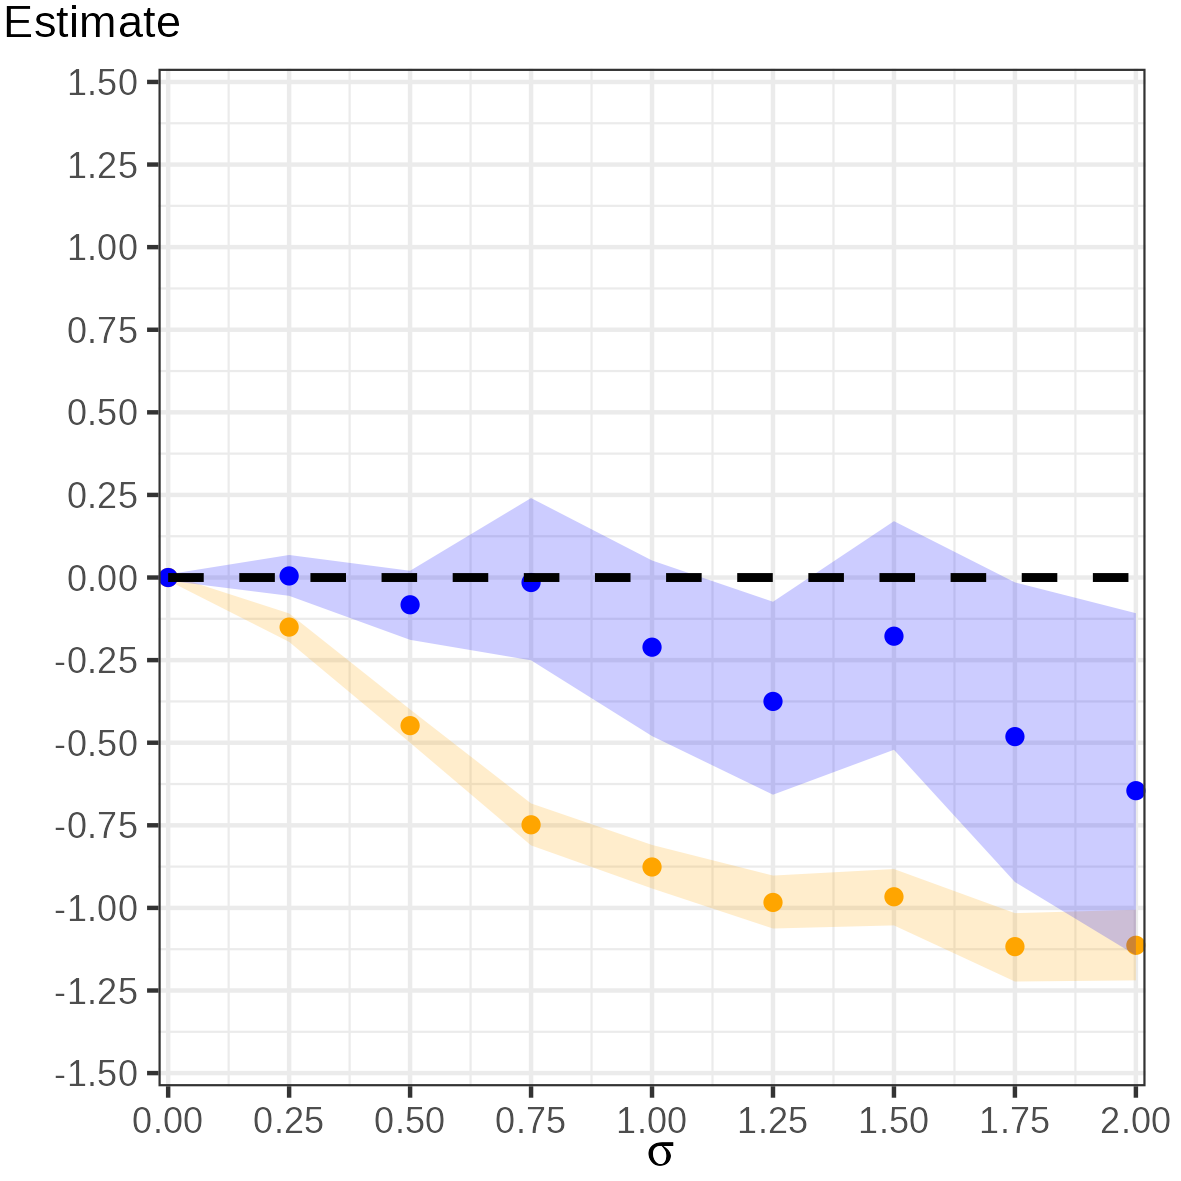
\includegraphics[width=\textwidth]{
            ../programs/simulations/sim-output/sigma-directeffect-bias.png}
    \end{subfigure}
    \begin{subfigure}[c]{0.475\textwidth}
        \centering
        \caption{$\hat{\text{AIE}} \;-$ AIE.}
        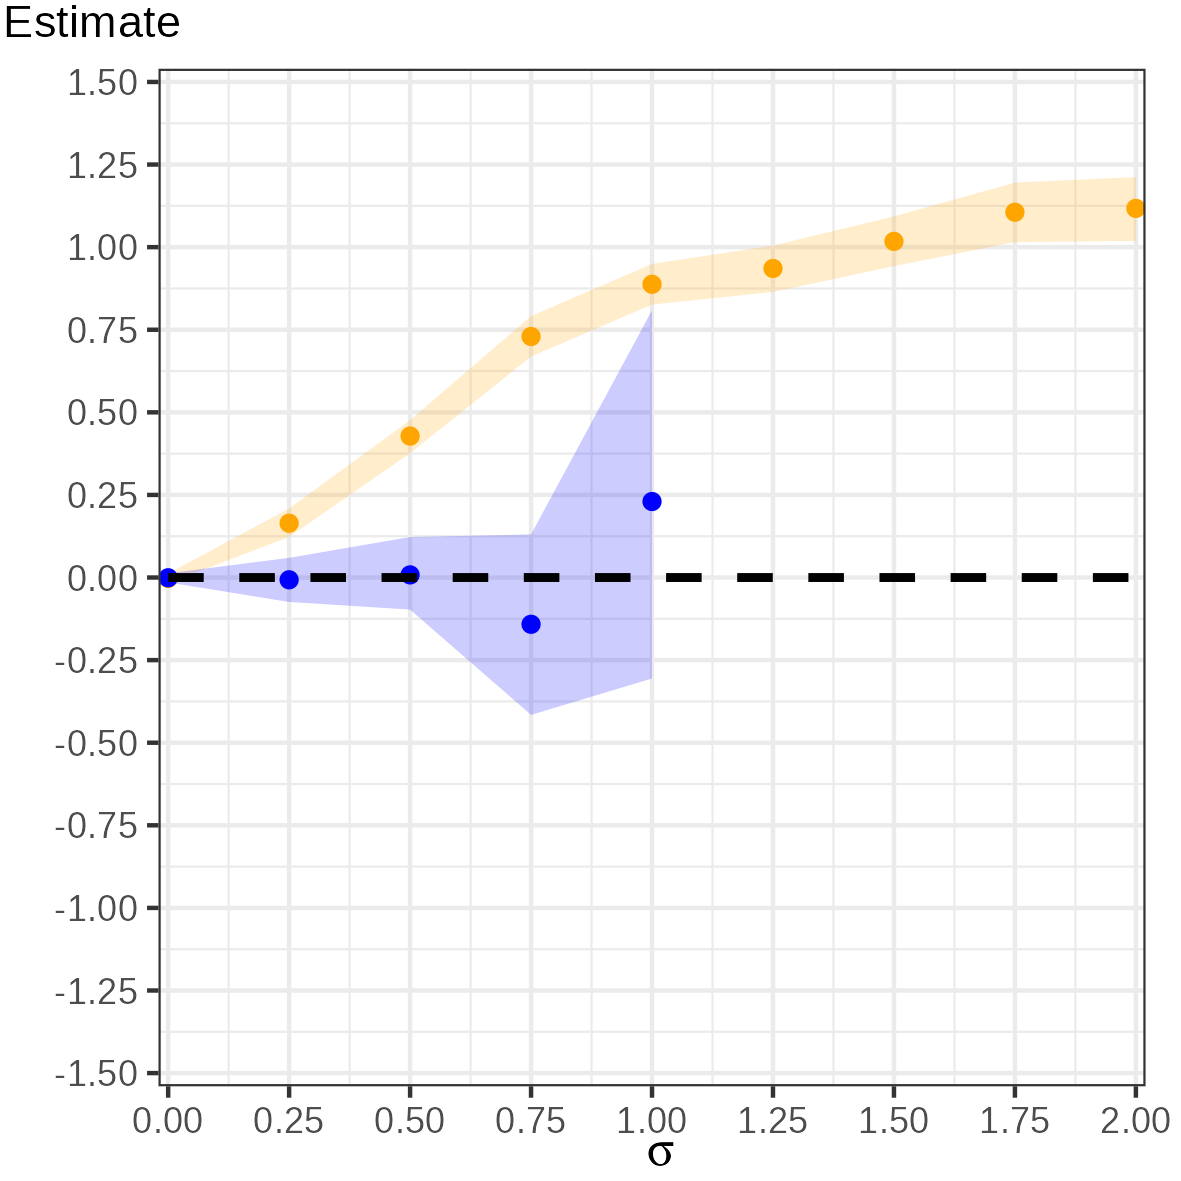
\includegraphics[width=\textwidth]{
            ../programs/simulations/sim-output/sigma-indirecteffect-bias.png}
    \end{subfigure}
    \label{fig:sigma-bias}
    \justify
    \footnotesize    
    \textbf{Note:}
    These figures show the OLS and control function point estimates of the ADE and AIE, for $N = 10,000$ sample size, minus the true value of the ADE and AIE, respectively.
    $y$-axis value of zero means the point estimate had estimated the ADE, or AIE, exactly.
    Points are points estimates from data simulated with a given $\rho = 0.5$ value, varying the $\sigma_0 = \sigma, \sigma_1 = 2\sigma$ values.
    Orange represents OLS estimates, blue the control function approach.
    Shaded regions are the 95\% confidence intervals from 1,000 bootstraps each.
\end{figure}

\begin{figure}[h!]
    \caption{OLS versus Control Function Estimates of CM Effects, varying $\sigma_1$ relative to $\sigma_0 = 1$.}
    \begin{subfigure}[c]{0.475\textwidth}
        \centering
        \caption{ADE.}
        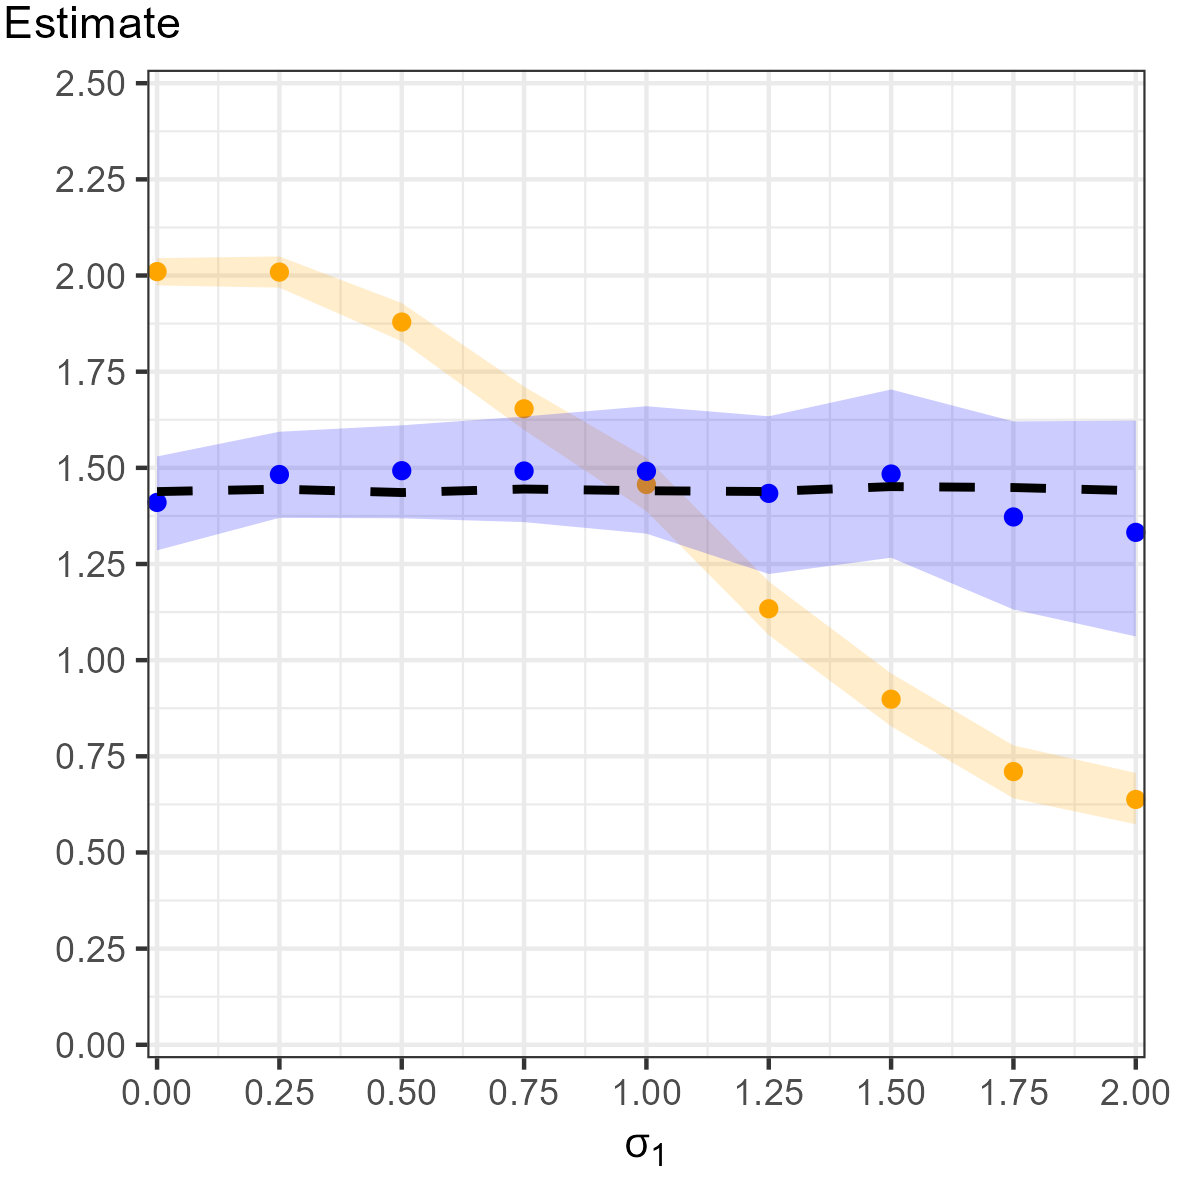
\includegraphics[width=\textwidth]{
            ../programs/simulations/sim-output/sigma-1-directeffect-bias.png}
    \end{subfigure}
    \begin{subfigure}[c]{0.475\textwidth}
        \centering
        \caption{AIE.}
        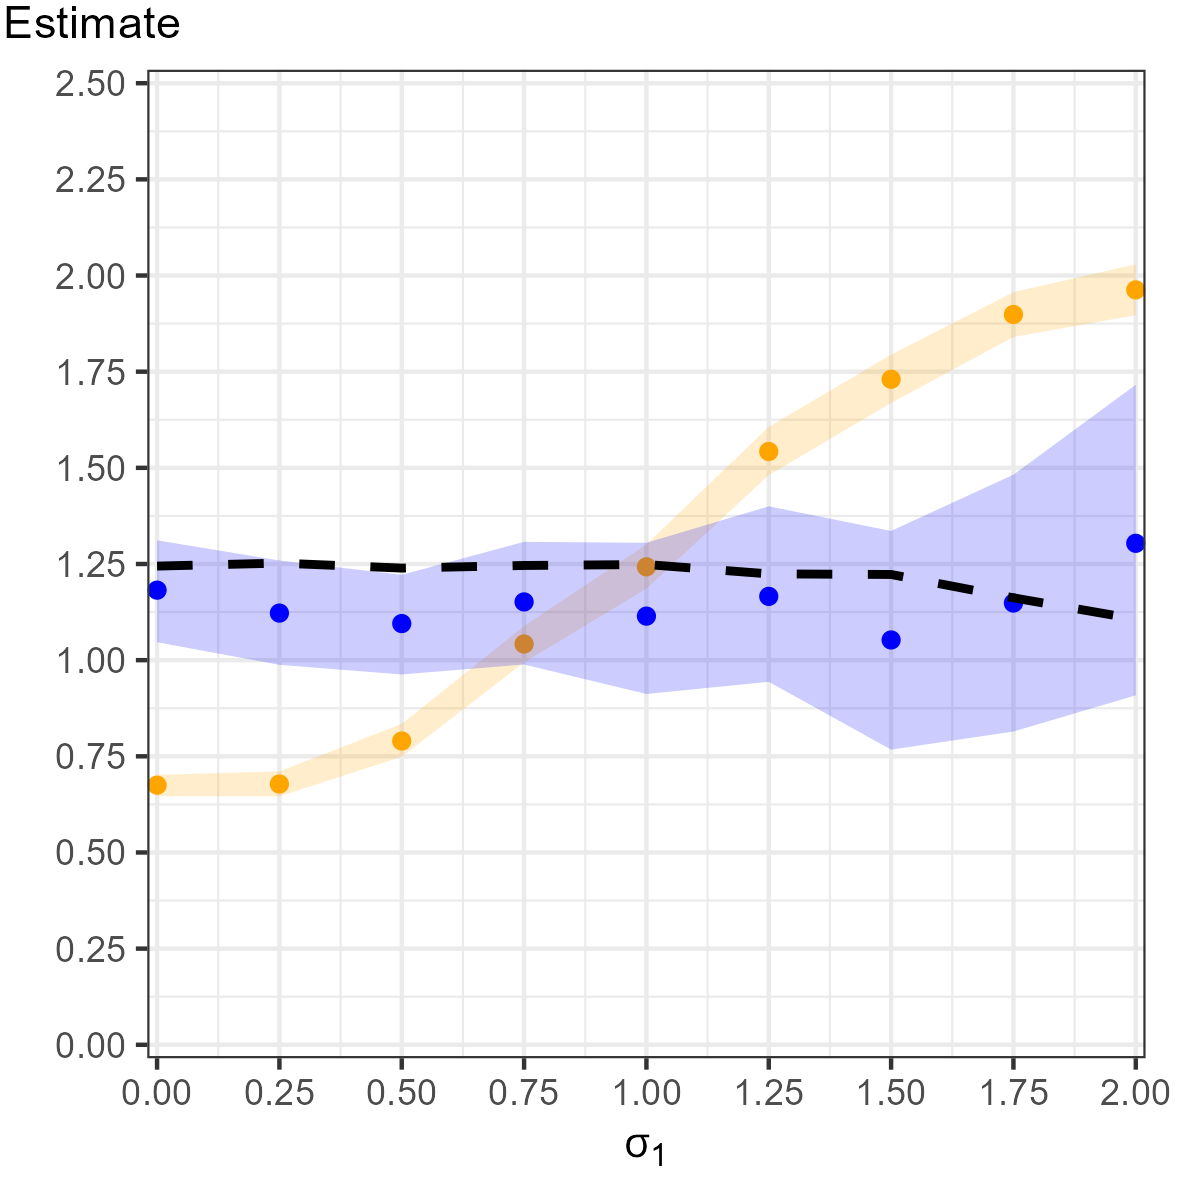
\includegraphics[width=\textwidth]{
            ../programs/simulations/sim-output/sigma-1-indirecteffect-bias.png}
    \end{subfigure}
    \label{fig:sigma-1-bias}
    \justify
    \footnotesize    
    \textbf{Note:}
    These figures show the OLS and control function estimates of the ADE and AIE, for $N = 10,000$ sample size.
    The black dashed line is the true value, points are points estimates from data simulated with a given $\rho = 0.5, \sigma_0 = 1$ and $\sigma_1$ varied across $[0, 2]$.
    Shaded regions are the 95\% confidence intervals;
    orange are the OLS estimates, blue the control function approach.
\end{figure}
